%
\documentclass[journal]{IEEEtran}
\usepackage{blindtext}
\usepackage{graphicx}
\usepackage{wrapfig}
\usepackage{textcomp}
\usepackage{dblfloatfix}
\usepackage{booktabs}
\usepackage{multirow}

%% or use the graphicx package for more complicated commands
\usepackage{gensymb}
%% or use the epsfig package if you prefer to use the old commands
%% \usepackage{epsfig}
% %\graphicspath{{D:/Studies/Internship/PS/Micro/Paper/Images}}
%% The amssymb package provides various useful mathematical symbols
\usepackage{amssymb}
%% The amsthm package provides extended theorem environments
%% \usepackage{amsthm}
\usepackage[cmex10]{amsmath}
\interdisplaylinepenalty=2500
\usepackage{cite}
\usepackage{color}
\usepackage{verbatim}


% Some very useful LaTeX packages include:
% (uncomment the ones you want to load)


\ifCLASSINFOpdf

\else
 
\fi
% correct bad hyphenation here
\hyphenation{op-tical net-works semi-conduc-tor}


\begin{document}
%
% paper title
% can use linebreaks \\ within to get better formatting as desired
\title{Learning Salient Objects in a Scene using Superpixel-augmented Convolutional Neural Network}
%
%
% author names and IEEE memberships
% note positions of commas and nonbreaking spaces ( ~ ) LaTeX will not break
% a structure at a ~ so this keeps an author's name from being broken across
% two lines.
% use \thanks{} to gain access to the first footnote area
% a separate \thanks must be used for each paragraph as LaTeX2e's \thanks
% was not built to handle multiple paragraphs
%

\author{Shashank~Tripathi\and, Yash Patel}


\markboth{}%
{Shell \MakeLowercase{\textit{et al.}}: Bare Demo of IEEEtran.cls for Journals}

% make the title area
\maketitle


\begin{abstract}
In this project, we are trying to determine salient objects in a scene. Salient objects are loosely defined as objects that “pop-out” in a scene in the opinion of a human observer -- an object that attracts attention of the human brain and visual system. 

Many previous studies have attempted to determine saliency in an image. This project specifically attempts to use Convolutional Neural Network to solve the binary labelling problem, where salient objects are labelled 1 and background is labelled 0. An obvious problem with using CNN directly is that CNNs use a highly low-resolution image as input (227x227 pixels for the popular Alexnet). Contrast based saliency should be detected from a larger context and such low resolutions put a cost on the context in the image. A solution is to cluster the image into Superpixels, which retain long-range context, while maintaining low-resolution input. Superpixel suffer from loss of spatial information, so we try to reinject spatial information by the incorporating the following observations: 
\begin{itemize}
	\item It has been shown in previous studies that contrast is a major factor to determine visual attention among humans	
	\item Another factor that determines visual attention is if the object is in the image foreground. Objects with contrast can occur scattered across the background, but foreground objects usually tend to be locally connected
\end{itemize}


\end{abstract}




% Note that keywords are not normally used for peerreview papers.
\begin{IEEEkeywords}
Saliency Detection, Convolutional Neural Networks, SLIC superpixels  
\end{IEEEkeywords}

\IEEEpeerreviewmaketitle

\section{Introduction}
\label{sec1}
“Thus, from the war of nature, from famine and death, the most exalted object which we are capable of conceiving, namely, the production of the higher animals, directly follows.” – On the Origin of Species, Charles Darwin. \\

Just as Charles Darwin attributed the success of all life on earth to a ubiquitous power called Evolution, we strongly believe that humans are only a biproduct of years of trial-and-error. The human visual system has developed over the years to optimally trade-off energy consumption and utility. It has been shown that the human visual system processes images in a hierarchical fashion [Marr and Poggio paper, 1982], starting from low-level context independent features like edges, contrast variation, color separation, etc to high-level features such as shape and structure. This observation has been instrumental in the development of the Convolutional Neural Networks which learn hierarchical weights in a similar fashion. This paper focuses on the use of low-level features to model human attention in a natural image.\\
 
Nassier et al (1964) proposed a model of the human visual system consisting of pre-attentive and attentive stages. The pre-attentive stage focuses human attention on “pop-out” features in the image. These “pop-out” features [Julesz, 1995] are regions in the image that present some form of spatial discontinuity, be it contrast separation or color variance. These features define Visual Saliency. Saliency detection is therefore an attempt to mimic the human visual system’s pre-attentive stage. In the context of this project, we try to use the power of convolutional neural networks to identify salient regions in an image. \\

Many past approaches at saliency detection try to capture contrast cues to determine salient regions [Cheng et al 2011, He and Lau 2014]. However, just as computer vision approaches using hand-crafted features have been shown to be unsuitable for a general setting, these approaches too fail to generalise to all images. Many researchers have therefore tried to adapt state-of-the-art learning techniques to detect salient regions but have primarily focused on integrating saliency maps obtained from hand-crafted features. {jiang et al, 2013]. This project takes inspiration from the results presented by the work of He et al, where they have tried to extract saliency labels on superpixels using a shallow Convolutional Neural Network. Using superpixels allow to reduce input dimension while retaining large image context. \\
	
Our approach:
    



\section{Dataset}

To train the Convolutional Neural Network, we have used the Extended Complex Scene Saliency dataset (ECSSD)[Heirarchical Saliency Detection, Yan et al] which provides 1000 natural images, along with ground truth labels. A few examples are shown in \ref{fig1}.
\begin{figure}[h]
	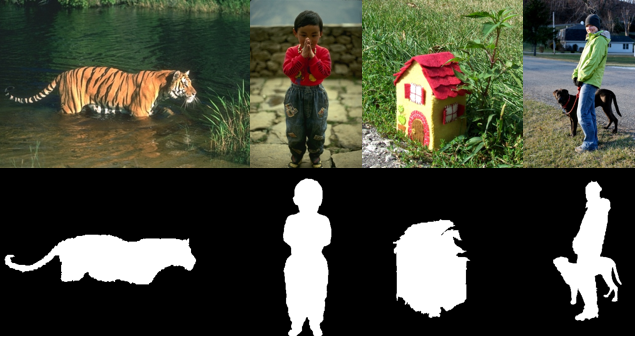
\includegraphics[width=1\linewidth]{dataset_img}
	\caption{Few sample image and corresponging ground truth labels from the ECSSD}
	\label{fig1}
\end{figure}



\section{Methodology}
\label{sec4}

An idea could be to directly feed the image pixels as input to a CNN architecture and generate saliency labels for each of the pixels. The issue with this approach is that most CNN architecture heavily downsample the input image (227x277 pixels for Alexnet, 224*244 pixels for VggNet and GoogleNet).  Such a small image patch is insufficient to detect saliency as saliency detection typically needs a larger image context. Low resolution puts a cost on the larger context in the image. The convolution operation also occurs in a 3x3 neighbourhood so as to capture local dependencies. While this might be useful for applications like image classification/ segmentation, which primarily rely on local information, saliency information is embedded globally. Local convolutions operation therefore fail to capture the global image context if directly applied on raw pixel values.\\

To mitigate the above issue, we propose using superpixel segmentation on the image. Humans don’t look at an image as a discretised matrix of pixels. To bridge the gap between how the human visual system perceives an image, many studies have proposed grouping pixels into perceptually meaningful regions that capture image redundancy. In general, superpixel regions have the following properties: \\
\begin{enumerate}
	\item Superpixels fit well to the object boundaries in the image
	\item Reduce pixelwise redundancies by grouping local pixels together based on color and intensity similarities
	\item Superpixels should be efficient to compute and should offer an efficiency advantage over and above their computation cost when used in a subsequent task
\end{enumerate}

Achanta et al have forwarded a powerful algorithm for superpixel segmentation called Simple Linear Iterative Clustering (SLIC). SLIC superpixels are based on the k-means clustering algorithm at its core. A simple modification that SLIC uses over the naïve k-means clustering is that it restricts the search space to a neighbourhood of the current mean. The neighbourhood is proportional to the superpixel size. This reduces the computational complexity to linear time (O(N)) where N are the number pixels are independent of the number of superpixels. Instead of taking Euclidean distance to propose cluster assignment, a color and spatial proximity based distance measure is used instead. The algorithm for SLIC superpixels can be summarised as below [Achanta et al]:\\

\begin{enumerate}
	\item Convert images from RGB colorspace to LAB colorspace \\
	
	CIE LAB colorspace bears a closer resemblance to human perception. It treats black and white as their own channel, i.e. it separates contrast from color, thereby having the advantage of a wider gamut. Contrast and color separation is important especially with regards to saliency detection as salient objects are localized based on both color and contrast separation in the context of the full image. 
	
	\item Write the rest of the algorithm from the slic superpixel paper. Describe the distance measure
\end{enumerate}

\ref{fig2} shows a few examples of superpixel segmentation on text images. It is apparent that the superpixels accurately group pixels based on color similarities. Moreover, superpixels adhere well to image boundaries.

An inherent problem with superpixel segmentation is that each time a different set of superpixels are generated stochastically depending upon the initial initialization of the cluster means. In the process, Superpixels lose spatial information. To recover spatial information, a color uniqueness matrix can be defined on the superpixels [He et al]. Let a give image \textit{I} and the segmented regions $ R = [r_1, \dots, r_x, \dots, r_N]^T $, a $N\times N\times 3$ color uniqueness matrix $Q$ can be defined. \\
\begin{align*}
Q = \begin{bmatrix}
q_{11}^c&\dots&q_{1j}^c&\dots&q_{1M}^c\\
\vdots&\ddots&&\ddots&\\
q_{x1}^c&\dots&q_{xj}^c&\dots&q_{xM}^c\\
\vdots&\ddots&&\ddots&\\
q_{N1}^c&\dots&q_{Nj}^c&\dots&q_{NM}^c
\end{bmatrix}
\end{align*}
where each element $q_{xj}^c$ represents the weighted difference in the mean color vector (across channels) of superpixel region $x$ with every other superpixel region $j$. So $M=N$ in our case.
\begin{align*}
q_{xj}^c = t(r_j).|C(r_x)-C(r_j)|.w(P(r_x),P(rj))
\end{align*}
where $t(r_j)$ counts the total number of pixels in region $r_j$. This term weights superpixels with more number of pixels to have higher contribution to the contrast than those with fewer pixels. $C(r_x)$ is the mean color vector of region $r_x$ and $|C(r_x)-C(r_j)|$ is the 3D vector storing absolute differences of each color channel. $P(r_x)$ is the mean position of $(r_x)$. The term $w(P(r_x),P(rj))$ is a Gaussian weight to attach higher contribution to pixels spatially closer to each other and $w(P(r_x),P(rj)) = exp(-\frac{1}{2\sigma_s^2}||P(r_x)-P(r_j)||^2$. Each row in Q is then sorted by the spatial distance to region $r_x$ to maintain local correlation such that the convolution operation in the CNN makes sense. Sorting groups neighbouring superpixels together. In summary, each row of the Q matrix describes the color differences between each region $r_X$ with all other M-1 superpixels in the image. The Gaussian distance weights include spatial information into the Q matrix which would have been lost otherwise. 

The color uniqueness matrix does a good job in capturing salient objects separated by color variations in the image. Q matrix essentially represents regions that show significant color rarity in their neighbourhood. However, considering just color rarity to determine saliency might be an oversimplification. Consider images in \ref{fig3} and their ground-truth salient object segmentations. It is apparent that even though certain objects display color rarity in the image eg. flowers, colored balls in the background, fishes etc, they are not salient. We need to ignore superpixels that display higher local contrast separation but form part of the background. Primarily, we need to a metric to differentiate foreground objects from background objects. [Lie et al, 2011] show that foreground objects are compact i.e. locally connected, whereas background objects are distributed in the image. To capture this difference, we define a new matrix $Q'$ which is complementary to the original $Q$ matrix.

\begin{figure}[h]
	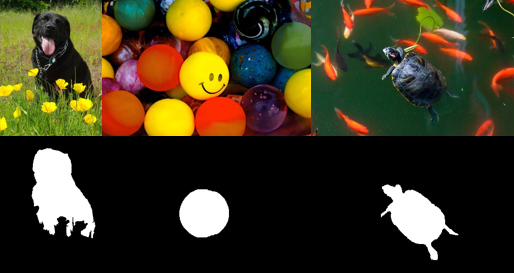
\includegraphics[width=1\linewidth]{scattered_background}
	\caption{Example of scattered non-salient background}
	\label{fig3}
\end{figure}   

\begin{align*}
Q' = \begin{bmatrix}
q_{11}^d&\dots&q_{1j}^d&\dots&q_{1M}^d\\
\vdots&\ddots&&\ddots&\\
q_{x1}^d&\dots&q_{xj}^d&\dots&q_{xM}^d\\
\vdots&\ddots&&\ddots&\\
q_{N1}^d&\dots&q_{Nj}^d&\dots&q_{NM}^d
\end{bmatrix}
\end{align*}
where each element $q;_{xj}^d$ represents the weighted difference in the mean position vector (across channels) of superpixel region $x$ with every other superpixel region $j$. Each $q_{xj}^d$ can be defined as: 
\begin{align*}
q_{xj}^d = t(r_j).|P(r_x)-P(r_j)|.w(C(r_x),C(rj))
\end{align*}
where $t(r_j)$ counts the total number of pixels in region $r_j$. This term weights superpixels with more number of pixels to have higher contribution to the contrast than those with fewer pixels. $P(r_x)$ is the mean position vector of region $r_x$ and $|P(r_x)-P(r_j)|$ is the 3D vector storing absolute differences of each color channel. $C(r_x)$ is the mean color of $(r_x)$ across the 3 channels. The term $w(C(r_x),C(rj))$ is a Gaussian weight to attach higher contribution to pixels spatially closer to each other in the color space and $w(C(r_x),C(rj)) = exp(-\frac{1}{2\sigma_s^2}||C(r_x)-C(r_j)||^2$. Each row in Q' is then sorted by the spatial distance to region $r_x$ to maintain local correlation such that the convolution operation in the CNN makes sense. This is similar to what we did while forming the Q matrix.

 



We look at saliency detection as a binary labeling problem where superpixels are classified as either salient or not. The relationship between the binary labellings and the Q matrix can be efficiently learned by a shallow Convolutional Neural Network. Salient objects display a perceptible difference in color compared to the surrounding and are locally connected. Our hypothesis is that the Q matrix accurately encompasses these properties of salient object from which a convolutional neural network can accurately learn internal representation to classify previously unseen images. 

\section{Network Architecture}
In this work, we use a shallow 3 stage Convolutional Neural Network with each stage having a 1D convolutional layer, a max-pooling operator, and a RELU activation. The first two stages include [] filters with kernel size 50 each. The architecure is summarized in \ref{fig4}.

\section{Experiments}
  
 



\begin{comment}
The overall pipeline flow is summarized in Fig. 1. Each step is further detailed in the following sections. \textcolor{red}{Should we remove Fig 1 altogether?}

\begin{figure}[h]
     \includegraphics[width=1\linewidth]{Images/pipeline_flow}
     \caption{Overview of proposed pipeline for classification of Alzheimer's disease}
\end{figure}

\subsection{Robex Brain Extraction}
\label{subsec4.0}

The first step in almost all MRI based classification pipelines is whole brain segmentation or skull stripping. Most previous studies have used methods such as Brain Extraction Tool (BET), Brain Surface Extraction (BSE), or FreeSurfer [“FreeSurfer,” online at http://surfer.nmr.mgh.harvard.edu.]. 
Although these methods perform well on certain datasets, a superior performance was observed using a more recent automatic brain segmentation procedure: Robust Brain Extraction (ROBEX)\cite{iglesias2011robust}. ROBEX doesn't require the user to tune any parameters specific to every subject and is thus especially useful for handling large datasets. ROBEX uses a combination of discriminative and generative model to fit the brain surface.  A shape model determines the fitting of a triangular mesh on the output of a supervised brain boundary classifier. It is more robust to case-specific structural deformations and provides a satisfactory performance on all patient scans used in this study.


\subsection{Atlas-based segmentation}
\label{subsec4.1}

 Studies that deal with more than 500 subjects typically find it tedious to perform manual segmentations. Manual segmentations are not only time and labor intensive but also require a high degree of repeatability. Typically, hippocampus segmentation itself takes between 30 min to 2 h to trace by hand \cite{carmichael2005atlas}. Therefore, more and more researchers are favouring atlas-based ROI segmentation approaches. Atlas-based segmentation is much more convenient, as it only require the user to align the atlas image with the subject image, and is well poised to take advantage of advances in image-to-image registration.
 
 In standard atlas-based segmentation methods, an `atlas', which contains pre-labelled manual tracings of brain ROIs, is registered to the subject image. The resulting spatial transformation is then used to map anatomical labels in the atlas to every individual subject. The approach used in this study registers each subject image to the MNI152 brain atlas. For registration, the FLIRT (FMRIB's Linear Image Registration Tool; http://fsl.fmrib.ox.ac.uk/fsl/fslwiki/FLIRT) was used which is part of the FMRIB Surface Library (FSL) package. We use the 12 dof affine registration with correlation ratio as cost function and trilinear interpolation method. The transformation matrix thus obtained is inversed to define a reverse transformation from MNI152 atlas space to subject space. This reverse transformation is then used to register AAL atlas, which is inherently in the MNI152 atlas space, to the subject space, thereby generating a subject-specific label for each ROI. A nearest neighbor interpolation strategy is used for reverse registration in order to preserve integral values of ROI labels. This strategy is implemented on 12 brain ROIs, shown in literature to be the most affected during AD progression. Fig. 2 delineates the 12 selected ROIs.
 
  \begin{figure}[h]
      \includegraphics[width=1\linewidth]{Images/rois}
      \caption{Selected ROIs}
 \end{figure}
 
 Collins et al.\cite{collins2010towards} use similar segmentation methods and have reported a dice kappa score of 0.844-0.874, a similarity of 0.729-0.776 and a normalised difference of 5.5\% for atlas-based hippocampal segmentations.
 
 In literature, many groups use FreeSurfer to obtain ROI segmentations and volume measures. It has been shown that Freesurfer boundaries, especially for hippocampus, are quite noisy, making them unsuitable for a detailed shape analysis.\cite{cong2014building}. Moreover, using Freesurfer, for ROI segmentation wasn't feasible given the large number of subjects used in this study. Freesurfer analysis tends to be extremely demanding in terms of both time and computational resources. Instead,  FIRST (http://www.fmrib.ox.ac.uk/fsl/fsl/list.html), the registration and segmentation tool in the FSL package, has recently become a tool of choice in several hippocampal shape studies. FIRST hippocampal segmentations are not only more accurate but also take lesser computational time. It was observed that FSL's FIRST yielded better hippocampal segmentations compared with our atlas-based approach. However, FSL provides segmentations only for sub-cortical regions necessitating the use of atlas-based approach for the remaining cortical ROI segmentations.
 
\subsection{Feature selection: Shape analysis using SPHARM PDM}
\label{subsubsec1}


Although volume as feature is intuitive and simple, shape analysis is considered to provide more accurate information pertaining to structural and anatomical changes. Global volume features fail to capture structural variations at specific locations. This study, thus, attempts to use shape features for achieving a better predictive accuracy.  

Spherical Harmonics (SPHARM) has been a popular approach to represent brain structures for shape analysis. A limitation of SPHARM, though, is that it can only represent objects of a spherical topology, limiting its application to sub-cortical brain structures such as the hippocampus and caudate. 

SPHARM takes binary hippocampus masks (obtained in the Section III(B)) as inputs. After initial processing to fill interior holes and a smoothing operation, the binary masks are converted to a surface mesh. A one-to-one, area-preserving, distortion minimizing  mapping is obtained between each point on the mesh and each point on a sphere by calculating a spherical parameterization\cite{brechbuhler1995parametrization}. The surface mesh \begin{math} v(\theta,\phi)=(x(\theta,\phi),y(\theta,\phi),z(\theta,\phi))^T \end{math} is decomposed using spherical harmonics basis functions and is represented as:

\begin{displaymath}
v(\theta,\phi)=\sum\limits_{l=0}^{\infty}\sum\limits_{m=-l}^{l}c_l^mY_l^m(\theta,\phi)
\end{displaymath}

where \(c_l^m\) represent three-dimensional vector coefficients due to the three coordinate functions and \(Y_l^m\) are spherical harmonic basis functions with degree l and order m; \(Y_l^m=\sqrt{\frac{(2l+1)(l-m)!}{4\pi(l+m)!}}P_l^m(cos\theta)e^im\phi.\) Here \( \theta\in[0,\pi],\ \phi\in[0,2\pi]\) and \(P_l^m\) are the associated Legendre polynomials. The SPHARM representation is transformed into a triangulated surface called SPHARM-PDM. A uniform subdivision of spherical parameterization results in each SPHARM-PDM having 1002 landmark coordinates. The SPHARM-PDM are spatially aligned using rigid procustes alignment. The alignment results in a one-to-one mapping between points of each surface mesh (SPHARM-PDM). The first NC subject is used as a template. We use the x, y, and z coordinates of the resulting SPHARM-PDM landmarks coordinates as features. 
 
In literature, some studies apply the corresponding rigid-body transform in the SPHARM decomposition resulting in new SPHARM coefficients. These coefficients are then used as features\cite{gerardin2009multidimensional}. We have tried to use the SPHARM landmark coordinates as features instead. The method of using implied PDM with SPHARM shape analysis was developed by Gerig et al.\cite{gerig2001shape} and has been used by Styner et al.\cite{styner2004correction} and Gerardin et al.\cite{gerardin2009multidimensional}.
 
 \begin{table*}[ht]
 \centering
 \begin{tabular*}{\textwidth}{l lllclllclllc @{}l}
 \toprule
 & \multicolumn{3}{l}{AD vs. NC} & & \multicolumn{3}{l}{AD vs. EMCI} &
  & \multicolumn{3}{l}{NC vs. LMCI}& &  \\
 \cmidrule{2-4} \cmidrule{6-8} \cmidrule{10-12}
 & ACC & SEN & SPE && ACC & SEN & SPE && ACC & SEN & SPE & & p-value\\ \midrule[0.2pt]
 I: Only VI & 83.41 & 73.43 & 88.52 && 83.21 & 77.61 & 87.96 && 71.11 & 65.35 & 76.08 & &\(\dagger/\dagger/\dagger\) \\
 II: Only SPHARM PDM coordinates & 78.12 & 4.72 & 98.83 && 73.59 & 39.24 & 87.21 && 68.86 & 65.21 & 71.14 & &\(\dagger/\dagger/\dagger\) \\
 III(a): Both VI and SPHARM (rbf SVM) & 85.98 & 75.55 & 90.30 && 84.59 & 81.06 & 86.67 && 71.91 & 71.52 & 72.24 & & n.a. \\
 III(b): Both VI and SPHARM (linear SVM) & 88.75 & 83.10 & 91.58 && 86.19 & 83.19 & 88.18 && 72.59 & 71.37 & 74.26 & & n.a \\ \midrule
 & \multicolumn{3}{l}{AD vs. LMCI} & & \multicolumn{3}{l}{NC vs. EMCI} &
  & \multicolumn{3}{l}{EMCI vs. LMCI}& &  \\
 \cmidrule{2-4} \cmidrule{6-8} \cmidrule{10-12}
 & ACC & SEN & SPE && ACC & SEN & SPE && ACC & SEN & SPE & & p-value\\ \midrule
 I: Only VI & 74.17 & 37.50 & 82.85 && 68.78 & 46.16 & 83.25 && 72.13 & 58.24 & 83.03 & &\(\dagger/\dagger/\dagger\) \\
 II: Only SPHARM PDM coordinates & 78.78 & 69.66 & 98.37 && 65.49 & 63.45 & 67.62 && 58.98 & 77.10 & 37.82 & &\(\dagger/0.01/0.575\) \\
 III(a): Both VI and SPHARM (rbf SVM) & 74.91 & 54.22 & 82.56 && 73.84 & 69.06 & 77.04 && 70.29 & 73.95 & 66.01 & & n.a. \\
 III(b): Both VI and SPHARM (linear SVM) & 76.81 & 79.79 & 74.21 && 75.46 & 74.03 & 76.63 && 70.95 & 75.56 & 65.47 & & n.a \\ 
 \bottomrule
 \end{tabular*}
 \caption{Classification accuracy (ACC), sensitivity (SEN), and specificity (SPE) (\%) values for methods I-III. Upper half lists performance metrics for the more diagnostically and structurally separated groups. More challenging sets are in the lower half. \(\dagger\) stands for p\(<\)0.001}
 \end{table*}
 


\subsection{Classification using SVM}
\label{subsubsec2}
After the feature selection step, we have a feature vector representation containing 12 mean voxel intensity values for each of the 12 ROIs and a shape feature matrix containing 6012 columns \{1002 (SPHARM PDM coordinates) * 3 (x,y,z) * 2 (both left and right hippocampus)\}. After variance weighing and mean centering, the shape feature dimension space was reduced by applying a principal component analysis (PCA) transformation.  Principal components were calculated such that 95\% of the group variance was retained.
 
A support vector machine (SVM) is a supervised classification method. Linear SVMs work by searching for the most optimal hyperplane separating data points of one class from the other. The most optimal hyperplane is the one with the largest margin between two classes and is found by solving the following optimization problem:
\begin{displaymath}
\min_{w,b,\xi}\frac{1}{2}w^T.w + C \sum\limits_{k=1}^{k}\xi^k 
\end{displaymath}
\begin{displaymath}
subject\ to \ y^k(w^T.x^k + b)\geq1-\xi^k; \ \xi^k\geq0
\end{displaymath}


where C is the cost parameter and \(\xi^k\) are positive slack variables allowing a soft margin. If the optimized classification function obtained thus is: \(f(x)=sign(x \cdot w+b)\)
such that w defines the orientation of the hyperplane and b defines the offset, it is seen that the classification function depends only on the dot products of the data. Non-linear separations can be created by replacing the dot product with a kernel evaluation. In this paper, we choose the radial basis function (rbf): \(K_\gamma(u,v)=e^{-\gamma||u-v||^2}\), where \(\gamma \) determines the width of the kernel. The performance of rbf kernel SVM was compared with linear SVM. 

\subsection{Validation}
\label{subsec3}
To obtain unbiased performance measures: accuracy (proportion of subjects classified correctly), sensitivity (true positive rate), and specificity (true negative rate), we use a 10-fold cross validation strategy. The whole subject cohort is randomly split into 10 subsets, of which 9 are used for training the SVM classifier and the remaining subset is used for test.  The process is successively repeated 10 times to avoid any possibility of bias. The training set is used to estimate optimal hyperparameters for rbf kernel SVM and to train the classifier.

To estimate the hyperparameters C and \(\gamma \), we use a two-fold grid search. In the coarse search,  values ranging between C = \(10^{-1} ...\ 10^7\) and \(\gamma=10^{-1}...\ 10^7\) are analyzed. A finer search is run on the most optimal C (C\(_{c-opt}\)) and \(\gamma\) (\(\gamma_{c-opt}\)),  obtained in the coarse grid search, with a range between 0.2 \(*\) C\(_{c-opt}\) to 8 \(*\) C\(_{c-opt}\) and 0.2 \(*\ \gamma_{c-opt}\) to 8 \(*\ \gamma_{c-opt}\). Both the coarse and fine grid search are repeated 5 times following the 5-fold cross-validation strategy. The C\(_{opt}\) and \(\gamma_{opt}\) yielding the maximum in-sample validation accuracy are chosen. The tuned hyperparameters are then used to predict the out-of-sample accuracy values on the test set. 

\section{Results and Discussion}
\label{sec5}

We run binary classification taking all possible combinations of classification problems: AD vs. NC, AD vs. EMCI, NC vs. LMCI, AD vs. LMCI, NC vs. EMCI and EMCI vs. LMCI. Accuracy, sensitivity and specificity values were averaged over 100 iterations. The validation strategy was repeated for the following methods: 
 \renewcommand{\labelenumi}{\Roman{enumi}}
\begin{enumerate}
\item Only Voxel Intensities as features
\item Only SPHARM PDM landmark coordinates 
\item Both VI and SPHARM coordinates 
\end{enumerate}
For testing the statistical significance of performance measures, unpaired t-tests are run between methods I-II and method III. For comparison, we train both linear and rbf kernel SVM. Table II summaries the performance metrics from our approach. As expected, the accuracy values are directly proportional to the morphological separation in brain scans giving the highest 89\% for NC vs. AD and 86\% for AD vs. EMCI. This observation is validated by maps of group differences shown in Fig. 3.  Shape analysis coupled with mean VIs give superior results as compared to only shape coordinates or only voxel intensities indicating that these features provide complementary information. 

 
 \begin{figure}[h]
      \includegraphics[width=1\linewidth]{Images/group_differences_1}
      \caption{Group differences between AD, LMCI, EMCI with normal controls }
 \end{figure}
 



In addition, the obtained results are comparable with or better than previously proposed approaches using MRI shape analysis. For instance, Suk et al.\cite{suk2013deep}, Goryawala et al.\cite{goryawala2015inclusion} and Wolz et al.\cite{wolz2012nonlinear} report NC vs. AD accuracy values of 85\%, 84\% and 88\%, respectively. Moreover, as opposed to our study, these studies rely on additional information from PET biomarkers or neuropsych test info.

Our approach performs especially well for the more challenging classification problems: NC vs. EMCI( 75.5\%), AD vs. LMCI(76.8\%) and EMCI vs. LMCI(71\%). Not many studies have explored shape analysis on classifying early and late mild cognitive impairment.  Gorywala et al.\cite{goryawala2015inclusion} do report accuracy values of 61.60\%, 59.60\% and 68.80\% for NC vs. EMCI, AD vs. LMCI and EMCI vs. LMCI, however, they don't use shape analysis. Cuignet et al.\cite{cuingnet2011automatic} use hippocampal shape analysis similar to our approach without adding voxel intensities, and report an accuracy of 84\% for NC vs. AD. Gerardin et al.\cite{gerardin2009multidimensional} follow a similar approach. However, they rely on SPHARM coefficients and analyze a much smaller cohort of 23 patients.

The results show that linear SVM is slightly superior than (or equal to) rbf SVM, indicating that the feature set is linearly separable.  Our algorithm outperforms strategies that use linearly inseparable feature set since linear SVM is faster than rbf SVM \textcolor{red}{Mahsa: it's wage. It outperforms in terms of speed you mean?}. Furthermore, the differences between accuracy values for NC vs AD reported in our paper and previously reported studies like Fan et al 2008\cite{fan2008structural} (94\%), and  Magnin et al\cite{magnin2009support} (94.5\%), may be due to the fact that such studies optimize hyperparameters on the testing set. This may lead to overfitting the test set\cite{cuingnet2011automatic}. Other studies that report superior results either use a different population cohort, other than ADNI, or use a relatively small number of subjects for analysis. Some studies\cite{goryawala2015inclusion} also try to include neuropsychological test scores\textcolor{red}{Mahsa: Goryawala used MMSE and CDR or tests like IQ scores?Because using IQ scores as feature for classification is meaningful} to enhance the classification performance. However, since ADNI labels patients' scans using test scores like CDR and MMSE, inclusion of test information in our feature set would mean training the SVM on clinical ground truth, undermining automatic feature extraction in our proposed CAD pipeline. 

 
\section{Conclusion}
\label{sec6}
In this paper, we present a novel automated CAD pipeline to classify patients into AD, LMCI, EMCI, and NC. Hippocampal shape features (SPHARM landmark coordinates) have been combined with mean voxel intensities for 12 selected ROIs to determine if these morphological features provide complementary information. We use a subject cohort of 600 subjects from the ADNI database. AAL atlas-based segmentation enables a convenient ROI segmentation. Both linear and rbf kernel SVM have been trained on the combined feature set and the results have been shown to be favorable as compared to conventional methods, especially for the more challenging classification problems: NC vs. EMCI, AD vs. LMCI and EMCI vs. LMCI. Future work will involve combining additional biomarkers such as cortical thickness data, volume, voxel-wise tissue probability, density of grey matter and multimodal data from imaging modalities such as PET-FDG and PET-AV45. 



\bibliographystyle{IEEEtran}
\bibliography{ref}
\end{comment}

\end{document}


